\documentclass[1p]{elsarticle_modified}
%\bibliographystyle{elsarticle-num}

%\usepackage[colorlinks]{hyperref}
%\usepackage{abbrmath_seonhwa} %\Abb, \Ascr, \Acal ,\Abf, \Afrak
\usepackage{amsfonts}
\usepackage{amssymb}
\usepackage{amsmath}
\usepackage{amsthm}
\usepackage{scalefnt}
\usepackage{amsbsy}
\usepackage{kotex}
\usepackage{caption}
\usepackage{subfig}
\usepackage{color}
\usepackage{graphicx}
\usepackage{xcolor} %% white, black, red, green, blue, cyan, magenta, yellow
\usepackage{float}
\usepackage{setspace}
\usepackage{hyperref}

\usepackage{tikz}
\usetikzlibrary{arrows}

\usepackage{multirow}
\usepackage{array} % fixed length table
\usepackage{hhline}

%%%%%%%%%%%%%%%%%%%%%
\makeatletter
\renewcommand*\env@matrix[1][\arraystretch]{%
	\edef\arraystretch{#1}%
	\hskip -\arraycolsep
	\let\@ifnextchar\new@ifnextchar
	\array{*\c@MaxMatrixCols c}}
\makeatother %https://tex.stackexchange.com/questions/14071/how-can-i-increase-the-line-spacing-in-a-matrix
%%%%%%%%%%%%%%%

\usepackage[normalem]{ulem}

\newcommand{\msout}[1]{\ifmmode\text{\sout{\ensuremath{#1}}}\else\sout{#1}\fi}
%SOURCE: \msout is \stkout macro in https://tex.stackexchange.com/questions/20609/strikeout-in-math-mode

\newcommand{\cancel}[1]{
	\ifmmode
	{\color{red}\msout{#1}}
	\else
	{\color{red}\sout{#1}}
	\fi
}

\newcommand{\add}[1]{
	{\color{blue}\uwave{#1}}
}

\newcommand{\replace}[2]{
	\ifmmode
	{\color{red}\msout{#1}}{\color{blue}\uwave{#2}}
	\else
	{\color{red}\sout{#1}}{\color{blue}\uwave{#2}}
	\fi
}

\newcommand{\Sol}{\mathcal{S}} %segment
\newcommand{\D}{D} %diagram
\newcommand{\A}{\mathcal{A}} %arc


%%%%%%%%%%%%%%%%%%%%%%%%%%%%%5 test

\def\sl{\operatorname{\textup{SL}}(2,\Cbb)}
\def\psl{\operatorname{\textup{PSL}}(2,\Cbb)}
\def\quan{\mkern 1mu \triangleright \mkern 1mu}

\theoremstyle{definition}
\newtheorem{thm}{Theorem}[section]
\newtheorem{prop}[thm]{Proposition}
\newtheorem{lem}[thm]{Lemma}
\newtheorem{ques}[thm]{Question}
\newtheorem{cor}[thm]{Corollary}
\newtheorem{defn}[thm]{Definition}
\newtheorem{exam}[thm]{Example}
\newtheorem{rmk}[thm]{Remark}
\newtheorem{alg}[thm]{Algorithm}

\newcommand{\I}{\sqrt{-1}}
\begin{document}

%\begin{frontmatter}
%
%\title{Boundary parabolic representations of knots up to 8 crossings}
%
%%% Group authors per affiliation:
%\author{Yunhi Cho} 
%\address{Department of Mathematics, University of Seoul, Seoul, Korea}
%\ead{yhcho@uos.ac.kr}
%
%
%\author{Seonhwa Kim} %\fnref{s_kim}}
%\address{Center for Geometry and Physics, Institute for Basic Science, Pohang, 37673, Korea}
%\ead{ryeona17@ibs.re.kr}
%
%\author{Hyuk Kim}
%\address{Department of Mathematical Sciences, Seoul National University, Seoul 08826, Korea}
%\ead{hyukkim@snu.ac.kr}
%
%\author{Seokbeom Yoon}
%\address{Department of Mathematical Sciences, Seoul National University, Seoul, 08826,  Korea}
%\ead{sbyoon15@snu.ac.kr}
%
%\begin{abstract}
%We find all boundary parabolic representation of knots up to 8 crossings.
%
%\end{abstract}
%\begin{keyword}
%    \MSC[2010] 57M25 
%\end{keyword}
%
%\end{frontmatter}

%\linenumbers
%\tableofcontents
%
\newcommand\colored[1]{\textcolor{white}{\rule[-0.35ex]{0.8em}{1.4ex}}\kern-0.8em\color{red} #1}%
%\newcommand\colored[1]{\textcolor{white}{ #1}\kern-2.17ex	\textcolor{white}{ #1}\kern-1.81ex	\textcolor{white}{ #1}\kern-2.15ex\color{red}#1	}

{\Large $\underline{11a_{129}~(K11a_{129})}$}

\setlength{\tabcolsep}{10pt}
\renewcommand{\arraystretch}{1.6}
\vspace{1cm}\begin{tabular}{m{100pt}>{\centering\arraybackslash}m{274pt}}
\multirow{5}{120pt}{
	\centering
	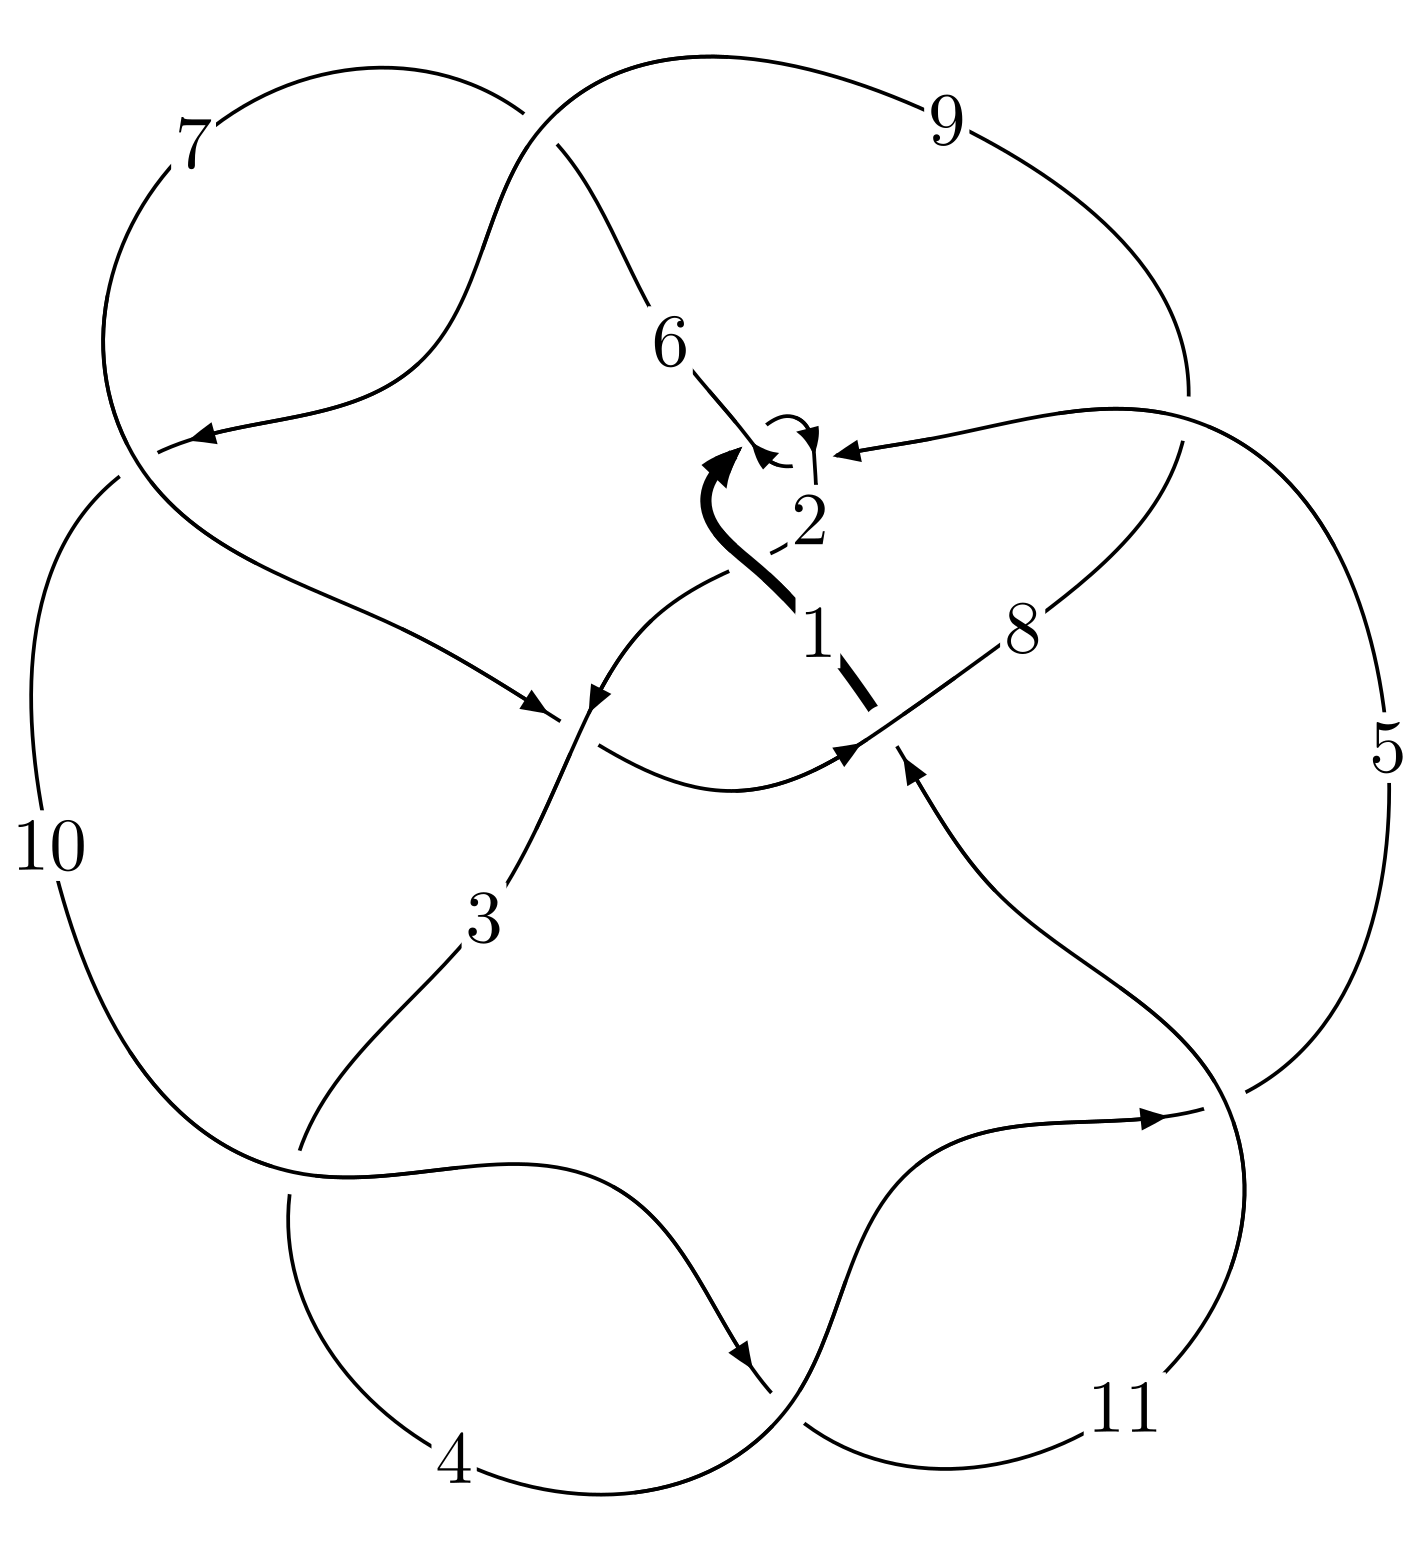
\includegraphics[width=112pt]{../../../GIT/diagram.site/Diagrams/png/378_11a_129.png}\\
\ \ \ A knot diagram\footnotemark}&
\allowdisplaybreaks
\textbf{Linearized knot diagam} \\
\cline{2-2}
 &
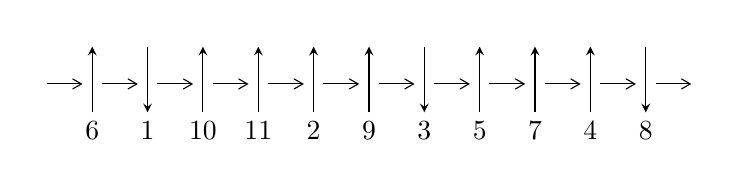
\begin{tikzpicture}[x=20pt, y=17pt]
	% nodes
	\node (C0) at (0, 0) {};
	\node (C1) at (1, 0) {};
	\node (C1U) at (1, +1) {};
	\node (C1D) at (1, -1) {6};

	\node (C2) at (2, 0) {};
	\node (C2U) at (2, +1) {};
	\node (C2D) at (2, -1) {1};

	\node (C3) at (3, 0) {};
	\node (C3U) at (3, +1) {};
	\node (C3D) at (3, -1) {10};

	\node (C4) at (4, 0) {};
	\node (C4U) at (4, +1) {};
	\node (C4D) at (4, -1) {11};

	\node (C5) at (5, 0) {};
	\node (C5U) at (5, +1) {};
	\node (C5D) at (5, -1) {2};

	\node (C6) at (6, 0) {};
	\node (C6U) at (6, +1) {};
	\node (C6D) at (6, -1) {9};

	\node (C7) at (7, 0) {};
	\node (C7U) at (7, +1) {};
	\node (C7D) at (7, -1) {3};

	\node (C8) at (8, 0) {};
	\node (C8U) at (8, +1) {};
	\node (C8D) at (8, -1) {5};

	\node (C9) at (9, 0) {};
	\node (C9U) at (9, +1) {};
	\node (C9D) at (9, -1) {7};

	\node (C10) at (10, 0) {};
	\node (C10U) at (10, +1) {};
	\node (C10D) at (10, -1) {4};

	\node (C11) at (11, 0) {};
	\node (C11U) at (11, +1) {};
	\node (C11D) at (11, -1) {8};
	\node (C12) at (12, 0) {};

	% arrows
	\draw[->,>={angle 60}]
	(C0) edge (C1) (C1) edge (C2) (C2) edge (C3) (C3) edge (C4) (C4) edge (C5) (C5) edge (C6) (C6) edge (C7) (C7) edge (C8) (C8) edge (C9) (C9) edge (C10) (C10) edge (C11) (C11) edge (C12) ;	\draw[->,>=stealth]
	(C1D) edge (C1U) (C2U) edge (C2D) (C3D) edge (C3U) (C4D) edge (C4U) (C5D) edge (C5U) (C6D) edge (C6U) (C7U) edge (C7D) (C8D) edge (C8U) (C9D) edge (C9U) (C10D) edge (C10U) (C11U) edge (C11D) ;
	\end{tikzpicture} \\
\hhline{~~} \\& 
\textbf{Solving Sequence} \\ \cline{2-2} 
 &
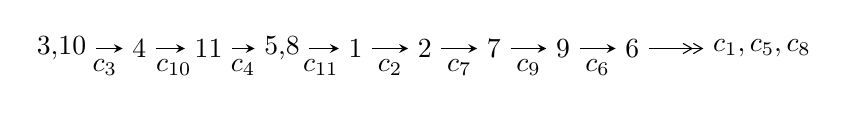
\begin{tikzpicture}[x=25pt, y=7pt]
	% node
	\node (A0) at (-1/8, 0) {3,10};
	\node (A1) at (1, 0) {4};
	\node (A2) at (2, 0) {11};
	\node (A3) at (49/16, 0) {5,8};
	\node (A4) at (33/8, 0) {1};
	\node (A5) at (41/8, 0) {2};
	\node (A6) at (49/8, 0) {7};
	\node (A7) at (57/8, 0) {9};
	\node (A8) at (65/8, 0) {6};
	\node (C1) at (1/2, -1) {$c_{3}$};
	\node (C2) at (3/2, -1) {$c_{10}$};
	\node (C3) at (5/2, -1) {$c_{4}$};
	\node (C4) at (29/8, -1) {$c_{11}$};
	\node (C5) at (37/8, -1) {$c_{2}$};
	\node (C6) at (45/8, -1) {$c_{7}$};
	\node (C7) at (53/8, -1) {$c_{9}$};
	\node (C8) at (61/8, -1) {$c_{6}$};
	\node (A9) at (10, 0) {$c_{1},c_{5},c_{8}$};

	% edge
	\draw[->,>=stealth]	
	(A0) edge (A1) (A1) edge (A2) (A2) edge (A3) (A3) edge (A4) (A4) edge (A5) (A5) edge (A6) (A6) edge (A7) (A7) edge (A8) ;
	\draw[->>,>={angle 60}]	
	(A8) edge (A9);
\end{tikzpicture} \\ 

\end{tabular} \\

\footnotetext{
The image of knot diagram is generated by the software ``\textbf{Draw programme}" developed by Andrew Bartholomew(\url{http://www.layer8.co.uk/maths/draw/index.htm\#Running-draw}), where we modified some parts for our purpose(\url{https://github.com/CATsTAILs/LinksPainter}).
}\phantom \\ \newline 
\centering \textbf{Ideals for irreducible components\footnotemark of $X_{\text{par}}$} 
 
\begin{align*}
I^u_{1}&=\langle 
3.90365\times10^{58} u^{58}+1.01441\times10^{59} u^{57}+\cdots+8.38498\times10^{58} b-3.01985\times10^{57},\\
\phantom{I^u_{1}}&\phantom{= \langle  }7.15963\times10^{59} u^{58}+1.21631\times10^{60} u^{57}+\cdots+9.22348\times10^{59} a-2.03520\times10^{59},\;u^{59}+2 u^{58}+\cdots+5 u^2-1\rangle \\
I^u_{2}&=\langle 
4 u^2+7 b+2 u-1,\;3 u^2+7 a+5 u+1,\;u^3+u^2-1\rangle \\
\\
\end{align*}
\raggedright * 2 irreducible components of $\dim_{\mathbb{C}}=0$, with total 62 representations.\\
\footnotetext{All coefficients of polynomials are rational numbers. But the coefficients are sometimes approximated in decimal forms when there is not enough margin.}
\newpage
\renewcommand{\arraystretch}{1}
\centering \section*{I. $I^u_{1}= \langle 3.90\times10^{58} u^{58}+1.01\times10^{59} u^{57}+\cdots+8.38\times10^{58} b-3.02\times10^{57},\;7.16\times10^{59} u^{58}+1.22\times10^{60} u^{57}+\cdots+9.22\times10^{59} a-2.04\times10^{59},\;u^{59}+2 u^{58}+\cdots+5 u^2-1 \rangle$}
\flushleft \textbf{(i) Arc colorings}\\
\begin{tabular}{m{7pt} m{180pt} m{7pt} m{180pt} }
\flushright $a_{3}=$&$\begin{pmatrix}1\\0\end{pmatrix}$ \\
\flushright $a_{10}=$&$\begin{pmatrix}0\\u\end{pmatrix}$ \\
\flushright $a_{4}=$&$\begin{pmatrix}1\\- u^2\end{pmatrix}$ \\
\flushright $a_{11}=$&$\begin{pmatrix}u\\- u^3+u\end{pmatrix}$ \\
\flushright $a_{5}=$&$\begin{pmatrix}- u^2+1\\u^4-2 u^2\end{pmatrix}$ \\
\flushright $a_{8}=$&$\begin{pmatrix}-0.776240 u^{58}-1.31871 u^{57}+\cdots-5.39605 u+0.220655\\-0.465552 u^{58}-1.20979 u^{57}+\cdots-0.0812092 u+0.0360150\end{pmatrix}$ \\
\flushright $a_{1}=$&$\begin{pmatrix}0.239979 u^{58}+0.405379 u^{57}+\cdots-1.25169 u-0.147253\\-0.137513 u^{58}-0.253368 u^{57}+\cdots-1.66158 u+0.0969722\end{pmatrix}$ \\
\flushright $a_{2}=$&$\begin{pmatrix}0.166747 u^{58}+0.266603 u^{57}+\cdots+0.146341 u+0.989129\\-0.000963728 u^{58}-0.0132996 u^{57}+\cdots+0.189286 u-0.00637696\end{pmatrix}$ \\
\flushright $a_{7}=$&$\begin{pmatrix}-1.24179 u^{58}-2.52850 u^{57}+\cdots-5.47726 u+0.256670\\-0.465552 u^{58}-1.20979 u^{57}+\cdots-0.0812092 u+0.0360150\end{pmatrix}$ \\
\flushright $a_{9}=$&$\begin{pmatrix}-1.16012 u^{58}-2.33933 u^{57}+\cdots-5.42935 u+0.193474\\-0.485917 u^{58}-1.19021 u^{57}+\cdots+1.07906 u+0.0222353\end{pmatrix}$ \\
\flushright $a_{6}=$&$\begin{pmatrix}-0.225910 u^{58}-0.512221 u^{57}+\cdots-0.169913 u+0.169646\\0.0153499 u^{58}-0.101739 u^{57}+\cdots-1.19569 u+0.0827941\end{pmatrix}$\\ \flushright $a_{6}=$&$\begin{pmatrix}-0.225910 u^{58}-0.512221 u^{57}+\cdots-0.169913 u+0.169646\\0.0153499 u^{58}-0.101739 u^{57}+\cdots-1.19569 u+0.0827941\end{pmatrix}$\\&\end{tabular}
\flushleft \textbf{(ii) Obstruction class $= -1$}\\~\\
\flushleft \textbf{(iii) Cusp Shapes $= -3.22898 u^{58}-6.33023 u^{57}+\cdots-0.906990 u+1.85953$}\\~\\
\newpage\renewcommand{\arraystretch}{1}
\flushleft \textbf{(iv) u-Polynomials at the component}\newline \\
\begin{tabular}{m{50pt}|m{274pt}}
Crossings & \hspace{64pt}u-Polynomials at each crossing \\
\hline $$\begin{aligned}c_{1},c_{5}\end{aligned}$$&$\begin{aligned}
&u^{59}-2 u^{58}+\cdots-4 u+1
\end{aligned}$\\
\hline $$\begin{aligned}c_{2}\end{aligned}$$&$\begin{aligned}
&u^{59}+24 u^{58}+\cdots+10 u-1
\end{aligned}$\\
\hline $$\begin{aligned}c_{3},c_{4},c_{10}\end{aligned}$$&$\begin{aligned}
&u^{59}-2 u^{58}+\cdots-5 u^2+1
\end{aligned}$\\
\hline $$\begin{aligned}c_{6},c_{9}\end{aligned}$$&$\begin{aligned}
&u^{59}+4 u^{58}+\cdots-257 u+49
\end{aligned}$\\
\hline $$\begin{aligned}c_{7}\end{aligned}$$&$\begin{aligned}
&7(7 u^{59}-22 u^{58}+\cdots-126239 u+81841)
\end{aligned}$\\
\hline $$\begin{aligned}c_{8}\end{aligned}$$&$\begin{aligned}
&7(7 u^{59}-6 u^{58}+\cdots+6234 u+1903)
\end{aligned}$\\
\hline $$\begin{aligned}c_{11}\end{aligned}$$&$\begin{aligned}
&u^{59}+5 u^{58}+\cdots-868 u+392
\end{aligned}$\\
\hline
\end{tabular}\\~\\
\newpage\renewcommand{\arraystretch}{1}
\flushleft \textbf{(v) Riley Polynomials at the component}\newline \\
\begin{tabular}{m{50pt}|m{274pt}}
Crossings & \hspace{64pt}Riley Polynomials at each crossing \\
\hline $$\begin{aligned}c_{1},c_{5}\end{aligned}$$&$\begin{aligned}
&y^{59}+24 y^{58}+\cdots+10 y-1
\end{aligned}$\\
\hline $$\begin{aligned}c_{2}\end{aligned}$$&$\begin{aligned}
&y^{59}+24 y^{58}+\cdots+462 y-1
\end{aligned}$\\
\hline $$\begin{aligned}c_{3},c_{4},c_{10}\end{aligned}$$&$\begin{aligned}
&y^{59}-60 y^{58}+\cdots+10 y-1
\end{aligned}$\\
\hline $$\begin{aligned}c_{6},c_{9}\end{aligned}$$&$\begin{aligned}
&y^{59}-50 y^{58}+\cdots+74183 y-2401
\end{aligned}$\\
\hline $$\begin{aligned}c_{7}\end{aligned}$$&$\begin{aligned}
&49(49 y^{59}+3394 y^{58}+\cdots-9.08304\times10^{10} y-6.69795\times10^{9})
\end{aligned}$\\
\hline $$\begin{aligned}c_{8}\end{aligned}$$&$\begin{aligned}
&49(49 y^{59}-64 y^{58}+\cdots+2.29562\times10^{8} y-3621409)
\end{aligned}$\\
\hline $$\begin{aligned}c_{11}\end{aligned}$$&$\begin{aligned}
&y^{59}+21 y^{58}+\cdots-2147376 y-153664
\end{aligned}$\\
\hline
\end{tabular}\\~\\
\newpage\flushleft \textbf{(vi) Complex Volumes and Cusp Shapes}
$$\begin{array}{c|c|c}  
\text{Solutions to }I^u_{1}& \I (\text{vol} + \sqrt{-1}CS) & \text{Cusp shape}\\
 \hline 
\begin{aligned}
u &= \phantom{-}0.622068 + 0.787958 I \\
a &= \phantom{-}0.481268 + 0.468907 I \\
b &= \phantom{-}0.71713 - 1.28444 I\end{aligned}
 & \phantom{-}4.44674 + 11.62550 I & \phantom{-0.000000 } 0 \\ \hline\begin{aligned}
u &= \phantom{-}0.622068 - 0.787958 I \\
a &= \phantom{-}0.481268 - 0.468907 I \\
b &= \phantom{-}0.71713 + 1.28444 I\end{aligned}
 & \phantom{-}4.44674 - 11.62550 I & \phantom{-0.000000 } 0 \\ \hline\begin{aligned}
u &= \phantom{-}0.506194 + 0.887762 I \\
a &= \phantom{-}0.672945 - 0.231781 I \\
b &= -0.249130 - 0.995558 I\end{aligned}
 & \phantom{-}4.02435 - 6.11409 I & \phantom{-0.000000 } 0 \\ \hline\begin{aligned}
u &= \phantom{-}0.506194 - 0.887762 I \\
a &= \phantom{-}0.672945 + 0.231781 I \\
b &= -0.249130 + 0.995558 I\end{aligned}
 & \phantom{-}4.02435 + 6.11409 I & \phantom{-0.000000 } 0 \\ \hline\begin{aligned}
u &= \phantom{-}0.857653 + 0.464032 I \\
a &= -0.033575 + 0.146733 I \\
b &= \phantom{-}0.707909 - 0.257892 I\end{aligned}
 & -1.83113 + 3.37489 I & \phantom{-0.000000 } 0. - 6.31964 I \\ \hline\begin{aligned}
u &= \phantom{-}0.857653 - 0.464032 I \\
a &= -0.033575 - 0.146733 I \\
b &= \phantom{-}0.707909 + 0.257892 I\end{aligned}
 & -1.83113 - 3.37489 I & \phantom{-0.000000 -}0. + 6.31964 I \\ \hline\begin{aligned}
u &= -0.627541 + 0.812622 I \\
a &= -0.518848 + 0.363833 I \\
b &= -0.548211 - 1.240870 I\end{aligned}
 & \phantom{-}6.17346 - 5.56581 I & \phantom{-0.000000 } 0 \\ \hline\begin{aligned}
u &= -0.627541 - 0.812622 I \\
a &= -0.518848 - 0.363833 I \\
b &= -0.548211 + 1.240870 I\end{aligned}
 & \phantom{-}6.17346 + 5.56581 I & \phantom{-0.000000 } 0 \\ \hline\begin{aligned}
u &= -0.970195\phantom{ +0.000000I} \\
a &= \phantom{-}0.167848\phantom{ +0.000000I} \\
b &= -0.593313\phantom{ +0.000000I}\end{aligned}
 & \phantom{-}1.61678\phantom{ +0.000000I} & \phantom{-}5.00000\phantom{ +0.000000I} \\ \hline\begin{aligned}
u &= -0.555862 + 0.900899 I \\
a &= -0.619428 - 0.061218 I \\
b &= \phantom{-}0.036940 - 1.051180 I\end{aligned}
 & \phantom{-}5.85876 - 0.11889 I & \phantom{-0.000000 } 0\\
 \hline 
 \end{array}$$\newpage$$\begin{array}{c|c|c}  
\text{Solutions to }I^u_{1}& \I (\text{vol} + \sqrt{-1}CS) & \text{Cusp shape}\\
 \hline 
\begin{aligned}
u &= -0.555862 - 0.900899 I \\
a &= -0.619428 + 0.061218 I \\
b &= \phantom{-}0.036940 + 1.051180 I\end{aligned}
 & \phantom{-}5.85876 + 0.11889 I & \phantom{-0.000000 } 0 \\ \hline\begin{aligned}
u &= \phantom{-}0.741521 + 0.922413 I \\
a &= \phantom{-}0.318033 + 0.111847 I \\
b &= \phantom{-}0.354088 - 0.782867 I\end{aligned}
 & -1.23742 + 3.26694 I & \phantom{-0.000000 } 0 \\ \hline\begin{aligned}
u &= \phantom{-}0.741521 - 0.922413 I \\
a &= \phantom{-}0.318033 - 0.111847 I \\
b &= \phantom{-}0.354088 + 0.782867 I\end{aligned}
 & -1.23742 - 3.26694 I & \phantom{-0.000000 } 0 \\ \hline\begin{aligned}
u &= \phantom{-}0.444629 + 0.510368 I \\
a &= -0.46434 - 1.56907 I \\
b &= -0.808317 + 0.689154 I\end{aligned}
 & -0.33205 + 6.44214 I & \phantom{-}4.62600 - 9.28024 I \\ \hline\begin{aligned}
u &= \phantom{-}0.444629 - 0.510368 I \\
a &= -0.46434 + 1.56907 I \\
b &= -0.808317 - 0.689154 I\end{aligned}
 & -0.33205 - 6.44214 I & \phantom{-}4.62600 + 9.28024 I \\ \hline\begin{aligned}
u &= \phantom{-}0.313615 + 0.597705 I \\
a &= -0.041562 - 1.003380 I \\
b &= -0.545415 + 0.167871 I\end{aligned}
 & -3.28171 + 0.39501 I & -2.00061 - 1.54672 I \\ \hline\begin{aligned}
u &= \phantom{-}0.313615 - 0.597705 I \\
a &= -0.041562 + 1.003380 I \\
b &= -0.545415 - 0.167871 I\end{aligned}
 & -3.28171 - 0.39501 I & -2.00061 + 1.54672 I \\ \hline\begin{aligned}
u &= -0.418675 + 0.447852 I \\
a &= \phantom{-}0.77452 - 1.30125 I \\
b &= \phantom{-}0.552817 + 0.774161 I\end{aligned}
 & \phantom{-}0.92823 - 1.58622 I & \phantom{-}7.27802 + 5.02607 I \\ \hline\begin{aligned}
u &= -0.418675 - 0.447852 I \\
a &= \phantom{-}0.77452 + 1.30125 I \\
b &= \phantom{-}0.552817 - 0.774161 I\end{aligned}
 & \phantom{-}0.92823 + 1.58622 I & \phantom{-}7.27802 - 5.02607 I \\ \hline\begin{aligned}
u &= -0.556478 + 0.207218 I \\
a &= \phantom{-}2.56199 - 0.99726 I \\
b &= -0.135387 + 0.940443 I\end{aligned}
 & \phantom{-}3.71804 - 4.17211 I & \phantom{-}12.3249 + 7.4178 I\\
 \hline 
 \end{array}$$\newpage$$\begin{array}{c|c|c}  
\text{Solutions to }I^u_{1}& \I (\text{vol} + \sqrt{-1}CS) & \text{Cusp shape}\\
 \hline 
\begin{aligned}
u &= -0.556478 - 0.207218 I \\
a &= \phantom{-}2.56199 + 0.99726 I \\
b &= -0.135387 - 0.940443 I\end{aligned}
 & \phantom{-}3.71804 + 4.17211 I & \phantom{-}12.3249 - 7.4178 I \\ \hline\begin{aligned}
u &= \phantom{-}0.559723 + 0.140117 I \\
a &= -2.77388 - 0.66591 I \\
b &= \phantom{-}0.244493 + 0.672850 I\end{aligned}
 & \phantom{-}4.05953 - 0.76565 I & \phantom{-}13.67462 - 0.08522 I \\ \hline\begin{aligned}
u &= \phantom{-}0.559723 - 0.140117 I \\
a &= -2.77388 + 0.66591 I \\
b &= \phantom{-}0.244493 - 0.672850 I\end{aligned}
 & \phantom{-}4.05953 + 0.76565 I & \phantom{-}13.67462 + 0.08522 I \\ \hline\begin{aligned}
u &= \phantom{-}0.423114 + 0.391843 I \\
a &= -0.472532 + 0.185081 I \\
b &= \phantom{-}0.957559 + 0.540672 I\end{aligned}
 & -0.25044 - 3.21979 I & \phantom{-}3.90025 + 0.90131 I \\ \hline\begin{aligned}
u &= \phantom{-}0.423114 - 0.391843 I \\
a &= -0.472532 - 0.185081 I \\
b &= \phantom{-}0.957559 - 0.540672 I\end{aligned}
 & -0.25044 + 3.21979 I & \phantom{-}3.90025 - 0.90131 I \\ \hline\begin{aligned}
u &= -1.42183 + 0.07250 I \\
a &= \phantom{-}1.57296 - 1.41800 I \\
b &= -1.32202 + 1.36648 I\end{aligned}
 & \phantom{-}5.48223 + 1.81992 I & \phantom{-0.000000 } 0 \\ \hline\begin{aligned}
u &= -1.42183 - 0.07250 I \\
a &= \phantom{-}1.57296 + 1.41800 I \\
b &= -1.32202 - 1.36648 I\end{aligned}
 & \phantom{-}5.48223 - 1.81992 I & \phantom{-0.000000 } 0 \\ \hline\begin{aligned}
u &= \phantom{-}1.44289 + 0.04366 I \\
a &= \phantom{-}0.12384 - 3.55457 I \\
b &= -0.75861 + 3.44954 I\end{aligned}
 & \phantom{-}6.34398 + 2.28663 I & \phantom{-0.000000 } 0 \\ \hline\begin{aligned}
u &= \phantom{-}1.44289 - 0.04366 I \\
a &= \phantom{-}0.12384 + 3.55457 I \\
b &= -0.75861 - 3.44954 I\end{aligned}
 & \phantom{-}6.34398 - 2.28663 I & \phantom{-0.000000 } 0 \\ \hline\begin{aligned}
u &= -1.44268 + 0.15844 I \\
a &= -0.095089 - 1.313110 I \\
b &= \phantom{-}0.121163 + 0.706508 I\end{aligned}
 & \phantom{-}2.38922 - 3.00723 I & \phantom{-0.000000 } 0\\
 \hline 
 \end{array}$$\newpage$$\begin{array}{c|c|c}  
\text{Solutions to }I^u_{1}& \I (\text{vol} + \sqrt{-1}CS) & \text{Cusp shape}\\
 \hline 
\begin{aligned}
u &= -1.44268 - 0.15844 I \\
a &= -0.095089 + 1.313110 I \\
b &= \phantom{-}0.121163 - 0.706508 I\end{aligned}
 & \phantom{-}2.38922 + 3.00723 I & \phantom{-0.000000 } 0 \\ \hline\begin{aligned}
u &= \phantom{-}1.45554 + 0.08236 I \\
a &= -0.41802 - 2.00373 I \\
b &= -0.05710 + 1.65402 I\end{aligned}
 & \phantom{-}6.50215 + 2.38989 I & \phantom{-0.000000 } 0 \\ \hline\begin{aligned}
u &= \phantom{-}1.45554 - 0.08236 I \\
a &= -0.41802 + 2.00373 I \\
b &= -0.05710 - 1.65402 I\end{aligned}
 & \phantom{-}6.50215 - 2.38989 I & \phantom{-0.000000 } 0 \\ \hline\begin{aligned}
u &= -1.48770\phantom{ +0.000000I} \\
a &= -0.815446\phantom{ +0.000000I} \\
b &= \phantom{-}1.74556\phantom{ +0.000000I}\end{aligned}
 & \phantom{-}8.30655\phantom{ +0.000000I} & \phantom{-0.000000 } 0 \\ \hline\begin{aligned}
u &= \phantom{-}1.49253 + 0.12922 I \\
a &= \phantom{-}0.04923 - 1.94060 I \\
b &= -0.422930 + 1.117500 I\end{aligned}
 & \phantom{-}7.23997 + 3.63562 I & \phantom{-0.000000 } 0 \\ \hline\begin{aligned}
u &= \phantom{-}1.49253 - 0.12922 I \\
a &= \phantom{-}0.04923 + 1.94060 I \\
b &= -0.422930 - 1.117500 I\end{aligned}
 & \phantom{-}7.23997 - 3.63562 I & \phantom{-0.000000 } 0 \\ \hline\begin{aligned}
u &= -1.49781 + 0.14706 I \\
a &= -0.27642 - 1.94523 I \\
b &= \phantom{-}0.530534 + 1.009310 I\end{aligned}
 & \phantom{-}6.06759 - 8.77463 I & \phantom{-0.000000 } 0 \\ \hline\begin{aligned}
u &= -1.49781 - 0.14706 I \\
a &= -0.27642 + 1.94523 I \\
b &= \phantom{-}0.530534 - 1.009310 I\end{aligned}
 & \phantom{-}6.06759 + 8.77463 I & \phantom{-0.000000 } 0 \\ \hline\begin{aligned}
u &= -1.52791 + 0.03503 I \\
a &= \phantom{-}0.720143 - 1.079900 I \\
b &= \phantom{-}0.482971 + 0.730580 I\end{aligned}
 & \phantom{-}11.01860 + 0.16153 I & \phantom{-0.000000 } 0 \\ \hline\begin{aligned}
u &= -1.52791 - 0.03503 I \\
a &= \phantom{-}0.720143 + 1.079900 I \\
b &= \phantom{-}0.482971 - 0.730580 I\end{aligned}
 & \phantom{-}11.01860 - 0.16153 I & \phantom{-0.000000 } 0\\
 \hline 
 \end{array}$$\newpage$$\begin{array}{c|c|c}  
\text{Solutions to }I^u_{1}& \I (\text{vol} + \sqrt{-1}CS) & \text{Cusp shape}\\
 \hline 
\begin{aligned}
u &= \phantom{-}1.52787 + 0.04986 I \\
a &= -0.71061 - 1.45487 I \\
b &= -0.434084 + 0.962095 I\end{aligned}
 & \phantom{-}10.66650 + 5.04841 I & \phantom{-0.000000 } 0 \\ \hline\begin{aligned}
u &= \phantom{-}1.52787 - 0.04986 I \\
a &= -0.71061 + 1.45487 I \\
b &= -0.434084 - 0.962095 I\end{aligned}
 & \phantom{-}10.66650 - 5.04841 I & \phantom{-0.000000 } 0 \\ \hline\begin{aligned}
u &= -0.304004 + 0.352318 I \\
a &= \phantom{-}0.725827 + 0.031622 I \\
b &= -0.401580 + 1.001260 I\end{aligned}
 & \phantom{-}0.818669 - 1.086870 I & \phantom{-}6.95263 + 5.92982 I \\ \hline\begin{aligned}
u &= -0.304004 - 0.352318 I \\
a &= \phantom{-}0.725827 - 0.031622 I \\
b &= -0.401580 - 1.001260 I\end{aligned}
 & \phantom{-}0.818669 + 1.086870 I & \phantom{-}6.95263 - 5.92982 I \\ \hline\begin{aligned}
u &= -0.336012 + 0.317334 I \\
a &= \phantom{-}1.151780 - 0.392616 I \\
b &= \phantom{-}0.165774 + 0.934262 I\end{aligned}
 & \phantom{-}0.674447 - 1.055540 I & \phantom{-}6.88917 + 6.16079 I \\ \hline\begin{aligned}
u &= -0.336012 - 0.317334 I \\
a &= \phantom{-}1.151780 + 0.392616 I \\
b &= \phantom{-}0.165774 - 0.934262 I\end{aligned}
 & \phantom{-}0.674447 + 1.055540 I & \phantom{-}6.88917 - 6.16079 I \\ \hline\begin{aligned}
u &= -1.57375 + 0.26330 I \\
a &= -0.02665 + 1.87772 I \\
b &= -0.97014 - 1.69830 I\end{aligned}
 & \phantom{-}11.6590 - 15.5089 I & \phantom{-0.000000 } 0 \\ \hline\begin{aligned}
u &= -1.57375 - 0.26330 I \\
a &= -0.02665 - 1.87772 I \\
b &= -0.97014 + 1.69830 I\end{aligned}
 & \phantom{-}11.6590 + 15.5089 I & \phantom{-0.000000 } 0 \\ \hline\begin{aligned}
u &= \phantom{-}1.57863 + 0.26847 I \\
a &= \phantom{-}0.12971 + 1.73446 I \\
b &= \phantom{-}0.85618 - 1.61480 I\end{aligned}
 & \phantom{-}13.4212 + 9.5497 I & \phantom{-0.000000 } 0 \\ \hline\begin{aligned}
u &= \phantom{-}1.57863 - 0.26847 I \\
a &= \phantom{-}0.12971 - 1.73446 I \\
b &= \phantom{-}0.85618 + 1.61480 I\end{aligned}
 & \phantom{-}13.4212 - 9.5497 I & \phantom{-0.000000 } 0\\
 \hline 
 \end{array}$$\newpage$$\begin{array}{c|c|c}  
\text{Solutions to }I^u_{1}& \I (\text{vol} + \sqrt{-1}CS) & \text{Cusp shape}\\
 \hline 
\begin{aligned}
u &= \phantom{-}1.59529 + 0.29735 I \\
a &= \phantom{-}0.350459 + 1.145760 I \\
b &= \phantom{-}0.534635 - 1.221130 I\end{aligned}
 & \phantom{-}12.98450 + 4.58039 I & \phantom{-0.000000 } 0 \\ \hline\begin{aligned}
u &= \phantom{-}1.59529 - 0.29735 I \\
a &= \phantom{-}0.350459 - 1.145760 I \\
b &= \phantom{-}0.534635 + 1.221130 I\end{aligned}
 & \phantom{-}12.98450 - 4.58039 I & \phantom{-0.000000 } 0 \\ \hline\begin{aligned}
u &= -1.60262 + 0.26158 I \\
a &= \phantom{-}0.106004 + 1.357480 I \\
b &= -0.94318 - 1.26607 I\end{aligned}
 & \phantom{-}6.48770 - 7.42956 I & \phantom{-0.000000 } 0 \\ \hline\begin{aligned}
u &= -1.60262 - 0.26158 I \\
a &= \phantom{-}0.106004 - 1.357480 I \\
b &= -0.94318 + 1.26607 I\end{aligned}
 & \phantom{-}6.48770 + 7.42956 I & \phantom{-0.000000 } 0 \\ \hline\begin{aligned}
u &= -1.59529 + 0.32218 I \\
a &= -0.428036 + 0.868477 I \\
b &= -0.397894 - 1.029760 I\end{aligned}
 & \phantom{-}10.90240 + 1.52833 I & \phantom{-0.000000 } 0 \\ \hline\begin{aligned}
u &= -1.59529 - 0.32218 I \\
a &= -0.428036 - 0.868477 I \\
b &= -0.397894 + 1.029760 I\end{aligned}
 & \phantom{-}10.90240 - 1.52833 I & \phantom{-0.000000 } 0 \\ \hline\begin{aligned}
u &= -0.046856 + 0.362935 I \\
a &= \phantom{-}0.240879 + 0.681944 I \\
b &= -0.04832 + 2.41526 I\end{aligned}
 & \phantom{-}2.15381 + 2.27881 I & -7.94357 + 3.32360 I \\ \hline\begin{aligned}
u &= -0.046856 - 0.362935 I \\
a &= \phantom{-}0.240879 - 0.681944 I \\
b &= -0.04832 - 2.41526 I\end{aligned}
 & \phantom{-}2.15381 - 2.27881 I & -7.94357 - 3.32360 I \\ \hline\begin{aligned}
u &= \phantom{-}0.349995\phantom{ +0.000000I} \\
a &= -2.41073\phantom{ +0.000000I} \\
b &= -0.734856\phantom{ +0.000000I}\end{aligned}
 & \phantom{-}2.11871\phantom{ +0.000000I} & \phantom{-}0.678540\phantom{ +0.000000I}\\
 \hline 
 \end{array}$$\newpage\newpage\renewcommand{\arraystretch}{1}
\centering \section*{II. $I^u_{2}= \langle 4 u^2+7 b+2 u-1,\;3 u^2+7 a+5 u+1,\;u^3+u^2-1 \rangle$}
\flushleft \textbf{(i) Arc colorings}\\
\begin{tabular}{m{7pt} m{180pt} m{7pt} m{180pt} }
\flushright $a_{3}=$&$\begin{pmatrix}1\\0\end{pmatrix}$ \\
\flushright $a_{10}=$&$\begin{pmatrix}0\\u\end{pmatrix}$ \\
\flushright $a_{4}=$&$\begin{pmatrix}1\\- u^2\end{pmatrix}$ \\
\flushright $a_{11}=$&$\begin{pmatrix}u\\u^2+u-1\end{pmatrix}$ \\
\flushright $a_{5}=$&$\begin{pmatrix}- u^2+1\\- u^2+u-1\end{pmatrix}$ \\
\flushright $a_{8}=$&$\begin{pmatrix}-\frac{3}{7} u^2-\frac{5}{7} u-\frac{1}{7}\\-\frac{4}{7} u^2-\frac{2}{7} u+\frac{1}{7}\end{pmatrix}$ \\
\flushright $a_{1}=$&$\begin{pmatrix}u\\u^2+u-1\end{pmatrix}$ \\
\flushright $a_{2}=$&$\begin{pmatrix}u\\2 u^2+u-2\end{pmatrix}$ \\
\flushright $a_{7}=$&$\begin{pmatrix}- u^2- u\\-\frac{4}{7} u^2-\frac{2}{7} u+\frac{1}{7}\end{pmatrix}$ \\
\flushright $a_{9}=$&$\begin{pmatrix}- u^2- u\\-\frac{4}{7} u^2+\frac{5}{7} u+\frac{1}{7}\end{pmatrix}$ \\
\flushright $a_{6}=$&$\begin{pmatrix}0\\- u\end{pmatrix}$\\ \flushright $a_{6}=$&$\begin{pmatrix}0\\- u\end{pmatrix}$\\&\end{tabular}
\flushleft \textbf{(ii) Obstruction class $= 1$}\\~\\
\flushleft \textbf{(iii) Cusp Shapes $= \frac{313}{49} u^2+\frac{188}{49} u+\frac{424}{49}$}\\~\\
\newpage\renewcommand{\arraystretch}{1}
\flushleft \textbf{(iv) u-Polynomials at the component}\newline \\
\begin{tabular}{m{50pt}|m{274pt}}
Crossings & \hspace{64pt}u-Polynomials at each crossing \\
\hline $$\begin{aligned}c_{1}\end{aligned}$$&$\begin{aligned}
&u^3+u^2+2 u+1
\end{aligned}$\\
\hline $$\begin{aligned}c_{2}\end{aligned}$$&$\begin{aligned}
&u^3+3 u^2+2 u-1
\end{aligned}$\\
\hline $$\begin{aligned}c_{3},c_{4}\end{aligned}$$&$\begin{aligned}
&u^3+u^2-1
\end{aligned}$\\
\hline $$\begin{aligned}c_{5}\end{aligned}$$&$\begin{aligned}
&u^3- u^2+2 u-1
\end{aligned}$\\
\hline $$\begin{aligned}c_{6}\end{aligned}$$&$\begin{aligned}
&(u+1)^3
\end{aligned}$\\
\hline $$\begin{aligned}c_{7}\end{aligned}$$&$\begin{aligned}
&7(7 u^3+u^2+u-1)
\end{aligned}$\\
\hline $$\begin{aligned}c_{8}\end{aligned}$$&$\begin{aligned}
&7(7 u^3- u^2-4 u-1)
\end{aligned}$\\
\hline $$\begin{aligned}c_{9}\end{aligned}$$&$\begin{aligned}
&(u-1)^3
\end{aligned}$\\
\hline $$\begin{aligned}c_{10}\end{aligned}$$&$\begin{aligned}
&u^3- u^2+1
\end{aligned}$\\
\hline $$\begin{aligned}c_{11}\end{aligned}$$&$\begin{aligned}
&u^3
\end{aligned}$\\
\hline
\end{tabular}\\~\\
\newpage\renewcommand{\arraystretch}{1}
\flushleft \textbf{(v) Riley Polynomials at the component}\newline \\
\begin{tabular}{m{50pt}|m{274pt}}
Crossings & \hspace{64pt}Riley Polynomials at each crossing \\
\hline $$\begin{aligned}c_{1},c_{5}\end{aligned}$$&$\begin{aligned}
&y^3+3 y^2+2 y-1
\end{aligned}$\\
\hline $$\begin{aligned}c_{2}\end{aligned}$$&$\begin{aligned}
&y^3-5 y^2+10 y-1
\end{aligned}$\\
\hline $$\begin{aligned}c_{3},c_{4},c_{10}\end{aligned}$$&$\begin{aligned}
&y^3- y^2+2 y-1
\end{aligned}$\\
\hline $$\begin{aligned}c_{6},c_{9}\end{aligned}$$&$\begin{aligned}
&(y-1)^3
\end{aligned}$\\
\hline $$\begin{aligned}c_{7}\end{aligned}$$&$\begin{aligned}
&49(49 y^3+13 y^2+3 y-1)
\end{aligned}$\\
\hline $$\begin{aligned}c_{8}\end{aligned}$$&$\begin{aligned}
&49(49 y^3-57 y^2+14 y-1)
\end{aligned}$\\
\hline $$\begin{aligned}c_{11}\end{aligned}$$&$\begin{aligned}
&y^3
\end{aligned}$\\
\hline
\end{tabular}\\~\\
\newpage\flushleft \textbf{(vi) Complex Volumes and Cusp Shapes}
$$\begin{array}{c|c|c}  
\text{Solutions to }I^u_{2}& \I (\text{vol} + \sqrt{-1}CS) & \text{Cusp shape}\\
 \hline 
\begin{aligned}
u &= -0.877439 + 0.744862 I \\
a &= \phantom{-}0.391708 + 0.028159 I \\
b &= \phantom{-}0.270651 + 0.534120 I\end{aligned}
 & -1.37919 - 2.82812 I & \phantom{-}6.66044 - 5.49186 I \\ \hline\begin{aligned}
u &= -0.877439 - 0.744862 I \\
a &= \phantom{-}0.391708 - 0.028159 I \\
b &= \phantom{-}0.270651 - 0.534120 I\end{aligned}
 & -1.37919 + 2.82812 I & \phantom{-}6.66044 + 5.49186 I \\ \hline\begin{aligned}
u &= \phantom{-}0.754878\phantom{ +0.000000I} \\
a &= -0.926273\phantom{ +0.000000I} \\
b &= -0.398445\phantom{ +0.000000I}\end{aligned}
 & \phantom{-}2.75839\phantom{ +0.000000I} & \phantom{-}15.1890\phantom{ +0.000000I}\\
 \hline 
 \end{array}$$\newpage
\newpage\renewcommand{\arraystretch}{1}
\centering \section*{ III. u-Polynomials}
\begin{tabular}{m{50pt}|m{274pt}}
Crossings & \hspace{64pt}u-Polynomials at each crossing \\
\hline $$\begin{aligned}c_{1}\end{aligned}$$&$\begin{aligned}
&(u^3+u^2+2 u+1)(u^{59}-2 u^{58}+\cdots-4 u+1)
\end{aligned}$\\
\hline $$\begin{aligned}c_{2}\end{aligned}$$&$\begin{aligned}
&(u^3+3 u^2+2 u-1)(u^{59}+24 u^{58}+\cdots+10 u-1)
\end{aligned}$\\
\hline $$\begin{aligned}c_{3},c_{4}\end{aligned}$$&$\begin{aligned}
&(u^3+u^2-1)(u^{59}-2 u^{58}+\cdots-5 u^2+1)
\end{aligned}$\\
\hline $$\begin{aligned}c_{5}\end{aligned}$$&$\begin{aligned}
&(u^3- u^2+2 u-1)(u^{59}-2 u^{58}+\cdots-4 u+1)
\end{aligned}$\\
\hline $$\begin{aligned}c_{6}\end{aligned}$$&$\begin{aligned}
&((u+1)^3)(u^{59}+4 u^{58}+\cdots-257 u+49)
\end{aligned}$\\
\hline $$\begin{aligned}c_{7}\end{aligned}$$&$\begin{aligned}
&49(7 u^3+u^2+u-1)(7 u^{59}-22 u^{58}+\cdots-126239 u+81841)
\end{aligned}$\\
\hline $$\begin{aligned}c_{8}\end{aligned}$$&$\begin{aligned}
&49(7 u^3- u^2-4 u-1)(7 u^{59}-6 u^{58}+\cdots+6234 u+1903)
\end{aligned}$\\
\hline $$\begin{aligned}c_{9}\end{aligned}$$&$\begin{aligned}
&((u-1)^3)(u^{59}+4 u^{58}+\cdots-257 u+49)
\end{aligned}$\\
\hline $$\begin{aligned}c_{10}\end{aligned}$$&$\begin{aligned}
&(u^3- u^2+1)(u^{59}-2 u^{58}+\cdots-5 u^2+1)
\end{aligned}$\\
\hline $$\begin{aligned}c_{11}\end{aligned}$$&$\begin{aligned}
&u^3(u^{59}+5 u^{58}+\cdots-868 u+392)
\end{aligned}$\\
\hline
\end{tabular}\newpage\renewcommand{\arraystretch}{1}
\centering \section*{ IV. Riley Polynomials}
\begin{tabular}{m{50pt}|m{274pt}}
Crossings & \hspace{64pt}Riley Polynomials at each crossing \\
\hline $$\begin{aligned}c_{1},c_{5}\end{aligned}$$&$\begin{aligned}
&(y^3+3 y^2+2 y-1)(y^{59}+24 y^{58}+\cdots+10 y-1)
\end{aligned}$\\
\hline $$\begin{aligned}c_{2}\end{aligned}$$&$\begin{aligned}
&(y^3-5 y^2+10 y-1)(y^{59}+24 y^{58}+\cdots+462 y-1)
\end{aligned}$\\
\hline $$\begin{aligned}c_{3},c_{4},c_{10}\end{aligned}$$&$\begin{aligned}
&(y^3- y^2+2 y-1)(y^{59}-60 y^{58}+\cdots+10 y-1)
\end{aligned}$\\
\hline $$\begin{aligned}c_{6},c_{9}\end{aligned}$$&$\begin{aligned}
&((y-1)^3)(y^{59}-50 y^{58}+\cdots+74183 y-2401)
\end{aligned}$\\
\hline $$\begin{aligned}c_{7}\end{aligned}$$&$\begin{aligned}
&2401(49 y^3+13 y^2+3 y-1)\\
&\cdot(49 y^{59}+3394 y^{58}+\cdots-90830373521 y-6697949281)
\end{aligned}$\\
\hline $$\begin{aligned}c_{8}\end{aligned}$$&$\begin{aligned}
&2401(49 y^3-57 y^2+14 y-1)\\
&\cdot(49 y^{59}-64 y^{58}+\cdots+229562386 y-3621409)
\end{aligned}$\\
\hline $$\begin{aligned}c_{11}\end{aligned}$$&$\begin{aligned}
&y^3(y^{59}+21 y^{58}+\cdots-2147376 y-153664)
\end{aligned}$\\
\hline
\end{tabular}
\vskip 2pc
\end{document}